\documentclass[12pt, titlepage]{article}

\usepackage{fullpage}
\usepackage[round]{natbib}
\usepackage{multirow}
\usepackage{booktabs}
\usepackage{tabularx}
\usepackage{graphicx}
\usepackage{float}
\usepackage{hyperref}
\usepackage{enumerate}
\usepackage{graphicx}
\hypersetup{
    colorlinks,
    citecolor=blue,
    filecolor=black,
    linkcolor=red,
    urlcolor=blue
}

%% Comments

\usepackage{color}

\newif\ifcomments\commentstrue %displays comments
%\newif\ifcomments\commentsfalse %so that comments do not display

\ifcomments
\newcommand{\authornote}[3]{\textcolor{#1}{[#3 ---#2]}}
\newcommand{\todo}[1]{\textcolor{red}{[TODO: #1]}}
\else
\newcommand{\authornote}[3]{}
\newcommand{\todo}[1]{}
\fi

\newcommand{\wss}[1]{\authornote{blue}{SS}{#1}} 
\newcommand{\plt}[1]{\authornote{magenta}{TPLT}{#1}} %For explanation of the template
\newcommand{\an}[1]{\authornote{cyan}{Author}{#1}}

%% Common Parts

\newcommand{\progname}{Software Engineering} % PUT YOUR PROGRAM NAME HERE
\newcommand{\authname}{Team 16, Durum Wheat Semolina
	\\ Alexander Moica
	\\ Yasmine Jolly
	\\ Jeffrey Wang
	\\ Jack Theriault
	\\ Catherine Chen
	\\ Justina Srebrnjak } % AUTHOR NAMES                 

\usepackage{hyperref}
    \hypersetup{colorlinks=true, linkcolor=blue, citecolor=blue, filecolor=blue,
                urlcolor=blue, unicode=false}
    \urlstyle{same}
                                


\newcounter{acnum}
\newcommand{\actheacnum}{AC\theacnum}
\newcommand{\acref}[1]{AC\ref{#1}}

\newcounter{ucnum}
\newcommand{\uctheucnum}{UC\theucnum}
\newcommand{\uref}[1]{UC\ref{#1}}

\newcounter{mnum}
\newcommand{\mthemnum}{M\themnum}
\newcommand{\mref}[1]{M\ref{#1}}

\begin{document}

\title{System Design for \progname{}} 
\author{\authname}
\date{\today}

\maketitle

\pagenumbering{roman}

\section{Revision History}

\begin{tabularx}{\textwidth}{p{3cm}p{2cm}X}
\toprule {\bf Date} & {\bf Version} & {\bf Notes}\\
\midrule
January 18, 2023 & 1.0 & Notes\\
%Date 2 & 1.1 & Notes\\
\bottomrule
\end{tabularx}

\newpage

\section{Reference Material}

This section records information for easy reference.
\subsection{Relevant Documentation}
This document references multiple other documents that are listed below:

\begin{itemize}
	\item SRS, \cite{SRS}
	\item Development Plan, \cite{DevelopmentPlan}
	\item MG, \cite{MG}
	\item MIS, \cite{MIS}
\end{itemize}

\subsection{Abbreviations and Acronyms}

\renewcommand{\arraystretch}{1.2}
\begin{tabular}{l l} 
  \toprule		
  \textbf{symbol} & \textbf{description}\\
  \midrule 
  \progname & Explanation of program name\\
  SRS & Software Requirements Specification\\
  MG & Module Guide\\
  MIS & Module Interface Specification\\
  %\wss{...} & \wss{...}\\
  \bottomrule
\end{tabular}\\

\newpage

\tableofcontents

\listoftables

\listoffigures

\newpage

\pagenumbering{arabic}

\section{Introduction}


\subsection{Document Purpose}

This series of design documents are comprised of the System Design document, 
the Module Guide, and the Module Interface Specification. The purpose of these 
documents is to communicate the modular decomposition of 
the Utrition application, and provide readers with information regarding the 
functions/methods of each module, as well as the relationships between modules. 
Information about the high-level decomposition of modules can be found in 
the \href{../SoftArchitecture/MG.pdf}{MG}.
Details regarding each module's functions and methods are discussed in 
the \href{../SoftDetailedDes/MIS.pdf}{MIS}.

\subsection{System Purpose}

The purpose of Utrition is to provide users with an application that empowers 
them to discover the nutritional value of the foods they are consuming, and track
their previously eaten meals. Utrition takes a unique approach to the traditional nutritional logging applications by providing a variety of ways for users to input their food items into the application. Users with keyboard-typing accessibility concerns will finally have a nutritional logging application that they can use without external assistance.

\wss{Users will be able to log their meals in a 
variety of ways, ranging from manual information entry, to image upload. 
Utrition will provide nutritional info based on the user's meals, and will 
allow users to access information on their past meals.}


\subsection{Scope}

Users will be able to input their food items to Utrition by using speech to text, typing, or uploading food images to the front-end user interface. If users would like to upload an image of the food they want nutritional information for, they would have to provide a photo of the food on the device using Utrition. This can be done by downloading an image of the food item from the internet, taking a photo on the device using Utrition, or by uploading a photo from the user's phone to the device using Utrition. After user input, Utrition will begin front-end and back-end calculations to obtain nutritional information for the food item from the public Nutritionix API. The nutritional information will be provided to the front-end user interface for the user to view.

\wss{Include a figure that show the System Context (showing the boundary between
your system and the environment around it.)}

\begin{figure}[H]
	\centering
	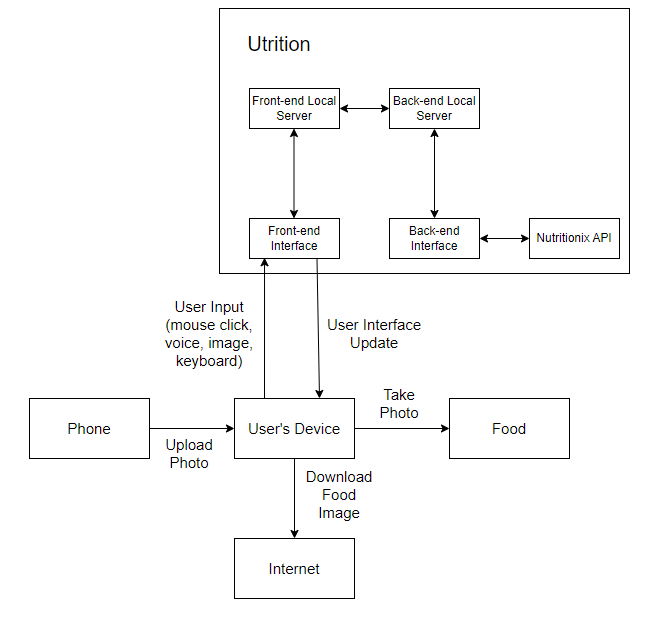
\includegraphics[scale=1]{System_Context_Diagram.png}
	\caption{System Context Diagram}
\end{figure}


\section{Project Overview}

\subsection{Normal Behaviour}

In their command-line interface, users will travel to the Utrition directory. From there, users will enter commands "npm start" and "npm run start-backend" separately. Utrition's front-end and back-end interfaces will successfully connect to the user's localhost server. Users will be greeted with the Utrition's home page. They may travel to their profile page, where they can find their past nutritional data saved in a list. On this page, users may decide to view their nutritional trends in graph form. Users may also travel to the upload page, where they can input food item(s) to find their nutritional information. Users can input food items by 
\begin{itemize}
	\item Clicking on the search bar and typing in the food items. Each food item is separated by a space.
	\item Clicking on the microphone button and verbally listing the food items.
	\item Clicking on the upload button and then selecting an image of a food item. Users can include multiple images in their search by clicking on the upload button again.
\end{itemize}
Users finalize their search by clicking the search button. In return, the user will be shown the nutritional information for each food item searched. The nutritional information is acquired from utilizing the Nutritionix public API. The data is stored on the user's device, so that past nutritional trends can be viewed on their profile page.

\subsection{Undesired Event Handling}

\wss{How you will approach undesired events}

A more in-depth look to Utrition's undesired event handling can be found in Utrition's \href{../../HazardAnalysis/HazardAnalysis.pdf}{Hazard Analysis} document.

In all cases except for one, the Utrition front-end interface will notify the user of the issue disrupting normal use of the application. Most of these errors will be detected by the back-end interface of Utrition. As a result, the application's back-end interface will send the error message to the front-end interface through the user's local server for the front-end interface to display. Certain errors, such as incorrect image type, are detected by the front-end interface and will not have to travel through the local servers to deliver the error message to the user. 

The one specific case where Utrition will not notify the user of the specific error is when Utrition closes unexpectedly. The cause of this rare issue is unknown to the developers, but the application will save its data periodically during use to ensure not much information is lost from the crash.

\subsection{Component Diagram}

\subsection{\href{../../SRS/SRS.pdf}{Connection Between Requirements and Design}} \label{SecConnection}

\wss{The intention of this section is to document decisions that are made
  ``between'' the requirements and the design.  To satisfy some requirements,
  design decisions need to be made.  Rather than make these decisions implicit,
  they are explicitly recorded here.  For instance, if a program has security
  requirements, a specific design decision may be made to satisfy those
  requirements with a password.}

\subsubsection{Functional Requirements}

\begin{enumerate}[{FR}1. ]
	\item Provide user a screen with the option to click a button, which then leads the user to upload an image.
	\item Provide the user a button to click on that allows them to enter another food item. After the second food item is entered, the button remains for more food items to be entered.
	\item The food item(s) uploaded to the Utrition front-end will be condensed to a 32x32 pixel image, which is then turned into a 32x32 array. The array containing data for each pixel is then transferred to the Utrition back-end. From there, the image is parsed through a TensorFlow machine learning algorithm which is trained on the CIFAR-100 dataset to determine the food item.
	\item The Utrition back-end provides the Nutritionix API with valid headers (x-app-id, x-app-key, x-remote-user-id) that allow the use of the API.
	\item The Utrition back-end interface sends a POST request to the Nutritionix API. The response to the POST request provides the back-end interface with a JSON file containing the food’s macro-nutrients, micro-nutrients, and caloric details.
	\item Once the Utrition back-end has received the nutritional details of the food item from the Nutritionix API, the back-end stores the nutritional information as a JSON file on the users’ Utrition folder.
	\item Once the user requests to see past nutritional data, the front-end interface sends a GET request to the front-end local server. This request is passed to the back-end local server, which then gets sent to the back-end interface. The back-end interface returns the data of all logged JSON files in the previously logged food items folder to the front-end interface (going through their respective local servers). The front-end interface displays the JSON files’ data in reverse-chronological order.
	\item Once the Utrition back-end interface receives the JSON file from the Nutritionix API, the data is sent to the local back-end server, to the local front-end server, and then to the front-end interface. In the front-end interface, the JSON file has the “stringify” method applied to it to display the information to the user.
	\item Once the user requests to see the past nutritional data graph, the front-end interface switches to a different user interface screen. From there, the front end interface sends a GET request to the front-end local server. This request is passed to the back-end local server, which then gets sent to the back-end interface. The back-end interface returns the data of all logged JSON files in the previously logged food items folder to the front-end interface (going through their respective local servers). The front-end interface parses the data by using ChartJS to display a graph of past nutritional trends to the user.
\end{enumerate}

\subsubsection{Non-Functional Requirements}
\begin{enumerate}[{LF}1. ]
	\item Front end developers will make a conscious effort not to place different components near each other. If components are determined to be close in proximity by the developers, \href{https://www.rapidtables.com/web/tools/pixel-ruler.html}{a pixel measuring tool} will be used to determine the distance between components.
\end{enumerate}

\begin{enumerate}[{UH}1. ]
	\item A navigation bar is provided at the top of every page.
	\item This design decision is covered by FR6's design decision.
	\item Utrition will provide steps on how to use the product on its homepage. Utrition will not provide the user with many available actions, so it becomes clear to individuals how to use the product. 
	\item Nutritional information (calories, fat, sodium, carbohydrates, sugar, and protein) will have an appropriate symbol next to it.
	\item Only important nutritional information is displayed to the user (calories, fat, sodium, carbohydrates, sugar, and protein) and back-end calculations are not displayed to the user. Front end reformatting of information will not be displayed to the user as well.
	\item No sound files will be found in Utrition's GitHub repository.
\end{enumerate}

\begin{enumerate}[{PR}1. ]
	\item Each screen loads in their personal set of functions. Each screen will not load in many functions.
	\item The machine learning algorithm sets the maximum amount of iterations to be 1000 for each image.
	\item No calculations are done while retrieving nutritional facts.
	\item The submitted image format is checked by the front-end interface, and if the image format is not “.png”, “.jpg”, or “.jpeg” an error message is returned to the user.
	\item The submitted image size is checked by the front-end interface, and if the image size is larger than 30MB an error message is returned to the user.
	\item After an image upload, the front-end interface counts the amount of images uploaded by the user. Once the amount of images exceeds 3, an error message is displayed to the user and the ability to proceed with the food-identification system is removed.
	\item Once the food image is sent to the back-end system, the machine learning algorithm begins a real-time stopwatch. After every iteration of the machine learning algorithm, the timer is checked. If the timer surpasses 10 seconds, an error message is sent to the back-end local server, which sends it to the front-end local server, which then sends it to the front-end interface to display the error message.
	\item Once the back-end determines the food item, a POST request is sent to the Nutrionix API. The Nutritionix API will send back a response, and the response is verified by the Utrition back-end system. If the response is “Too many requests”, the user cannot submit more food items. Once an error message is detected by the Utrition back-end system, the message is sent to the back-end local server, which sends it to the front-end local server, which then sends it to the front-end interface to display the error message.
	\item Once the back-end determines the food item, a POST request is sent to the Nutrionix API. The Nutritionix API will send back a response, and the response is verified by the Utrition back-end system. If the response is empty, the food item was not found in the Nutrionix API. The response is sent to the back-end local server, which sends it to the front-end local server, which then sends it to the front-end interface to display the error message.
	\item After the back-end interface determines that the past nutritional logs folder is empty, the back-end returns an error message to the front-end interface's GET request through their respective local servers. The front-end interface displays the error message to the user.
	\item If the back-end interface cannot find the past nutritional logs folder because it has been moved/deleted, the back-end returns an error message to the front-end interface's GET request through their respective local servers. The front-end interface displays the error message to the user.
	\item Once the user requests the past foods graph to be displayed. The front-end system sends a request to the front-end local server, which travels to the back-end local server to the back-end system. If the back-end system cannot find any stored data, an error message is sent back to the local back-end server, which travels to the local front-end server to the front-end system. The error message is displayed to the user in the front-end interface.
	\item Once the back-end determines the food item, a POST request is sent to the Nutrionix API. The Nutritionix API will send back a response, and the response is verified by the Utrition back-end system. If the response is a timed-out error, the user has an issue with their internet connection. Once an error message is detected by the Utrition back-end system, the message is sent to the back-end local server, which sends it to the front-end local server, which then sends it to the front-end interface to display the error message.
	\item The learning rate of the machine learning algorithm is set to 0.005.
	\item The Nutritionix API will provide correct results to the back-end, which then gets sent to the front-end interface through their respective local servers unless the user does not have an internet connection or an obscure food item is entered.
	\item Utrition is a local web application.
	\item After an image upload, the front-end interface counts the amount of images uploaded by the user. Once the amount of images exceeds 3, an error message is displayed to the user and the ability to proceed with the food-identification system is removed.
	\item Utrition is a local web application.
	\item Utrition is available on GitHub.
\end{enumerate}

\begin{enumerate}[{OE}1. ]
	\item Utrition is available on GitHub.
	\item The installation guide on GitHub is written in simple English.
	\item No developers will make changes to Utrition after publication.
\end{enumerate}

\begin{enumerate}[{MS}1. ]
	\item The CIFAR-100 dataset can be swapped with another appropriate dataset by placing it under the src/utrition-backend/ML/ folder.
	\item Developers will upload an installation guide, and a guide on how to use the web application on the Utrition GitHub.
	\item This design decision is covered by PR4's design decision.
\end{enumerate}

\begin{enumerate}[{SR}1. ]
	\item Utrition is available on GitHub.
	\item This design decision is covered by FR6's design decision.
	\item Utrition only stores previously searched food items’ nutritional information on the users’ Utrition folder. Utrition does not communicate with other instances of Utrition on other devices.
\end{enumerate}

\begin{enumerate}[{CP}1. ]
	\item Developers will not include any potentially insensitive content.
\end{enumerate}	

\begin{enumerate}[{LR}1. ]
	\item Developers will not include any malicious software in Utrition.
	\item Development of Utrition will be done on GitHub.
	\item GitHub’s CI/CD pipeline will be used with Pylint. Developers will review the results of the Pylint test to determine if coding conventions are not being followed properly.
	\item Front-end developers code in HTML and CSS using Google’s style guide. A review is performed by the front-end developers before the final launch of Utrition.
	\item Front-end developers design the interface using Google’s style guide. A review is performed by the front-end developers before the final launch of Utrition.
\end{enumerate}	
\section{System Variables}

\wss{Include this section for Mechatronics projects}

\subsection{Monitored Variables}

N/A

\subsection{Controlled Variables}

N/A

\subsection{Constants Variables}

N/A

\section{User Interfaces}

\wss{Design of user interface for software and hardware.  Attach an appendix if
needed. Drawings, Sketches, Figma}

\section{Design of Hardware}

\wss{Most relevant for mechatronics projects}
\wss{Show what will be acquired}
\wss{Show what will be built, with detail on fabrication and materials}
\wss{Include appendices as appropriate, possibly with sketches, drawings, CAD, 
etc}

N/A

\section{Design of Electrical Components}

\wss{Most relevant for mechatronics projects}
\wss{Show what will be acquired}
\wss{Show what will be built, with detail on fabrication and materials}
\wss{Include appendices as appropriate, possibly with sketches, drawings,
circuit diagrams, etc}

N/A

\section{Design of Communication Protocols}

\wss{If appropriate}

To use Utrition users must run commands “npm start” and “npm run start-backend”. The “npm start” command allows for the front-end user interface to be displayed and connects the front-end interface to the user’s local server (http://localhost:3000). The “npm run start-backend” command creates an unseen back-end interface on the user’s local server (http://localhost:5000). Since the front-end and back-end connect to the same local server with different ports, communication is done by the front-end sending GET and POST requests to the front-end local server, which is then read by the connecting back-end local server. The back-end interface receives the GET or POST request from the back-end local server and begins working on the given task. Once the task has been completed, the back-end returns data through the local server to reach the front-end (which is waiting for the back-end’s response). For example, if the request from the front-end is to find nutritional data for a food item, the front-end will send a GET request to the local server. The back-end reads this GET request from their local server (because they are located at the same address) and sends a POST request to the Nutritionix API. In return, the Nutritionix API will deliver the data back to the back-end. From there, the back-end returns the Nutritional data to the front-end by using the local server. 


\section{Timeline}

\wss{Schedule of tasks and who is responsible}

\bibliographystyle {plainnat}
\bibliography{../../../refs/References}

\newpage{}

\appendix

\section{Interface}

\wss{Include additional information related to the appearance of, and
interaction with, the user interface}

\section{Mechanical Hardware}

N/A

\section{Electrical Components}

N/A

\section{Communication Protocols}

\begin{figure}[H]
	\centering
	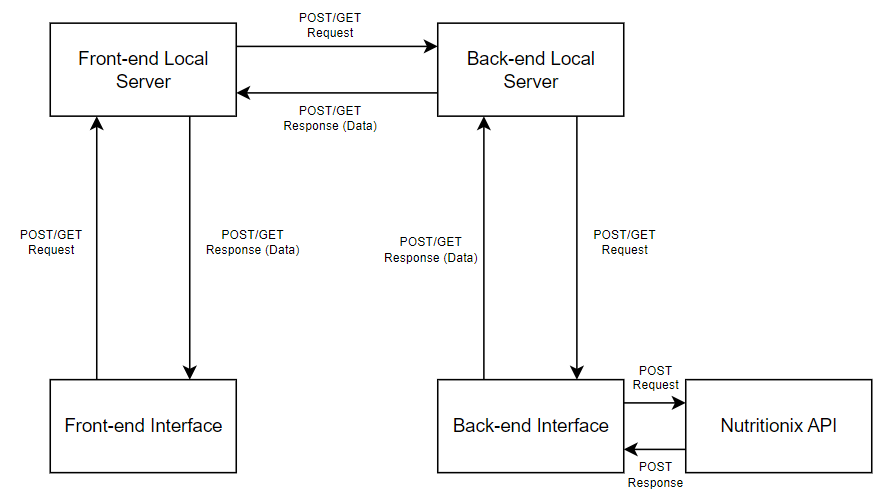
\includegraphics[scale=0.85]{Communication_Protocols.png}
	\caption{Communication between the front-end and back-end}
\end{figure}

\section{Reflection}

The information in this section will be used to evaluate the team members on the
graduate attribute of Problem Analysis and Design.  Please answer the following questions:

\begin{enumerate}
  \item What are the limitations of your solution?  Put another way, given
  unlimited resources, what could you do to make the project better? (LO\_ProbSolutions)
  \item Give a brief overview of other design solutions you considered.  What
  are the benefits and tradeoffs of those other designs compared with the chosen
  design?  From all the potential options, why did you select documented design?
  (LO\_Explores)
\end{enumerate}

Utrition utilizes the CIFAR-100 dataset to identify food items with TensorFlow, a machine learning algorithm. However, the CIFAR-100 dataset only contains 5 identifiable food items. With unlimited resources, the Utrition team would find a larger dataset containing most generic food items. With this larger dataset, the developers would have to change the machine learning model to accept the new data entries. Furthermore, with unlimited resources/time, the front end developers will have more time to tinker with stylistic choices to see which style works better for the Utrition application. Most notably, the front end developers would add charts and diagrams to display a user's previous meals rather than listing them.

The original design for Utrition was to only utilize machine learning models. Using only one method to search food items ensured a streamlined process for simplicity and a clutterless interface. However the tradeoff was that complex food items, such as a McDonald's Junior Chicken, would be impossible for a machine to identify. As a result, users would quickly get frustrated with the near-useless application. Therefore, the developers behind Utrition decided that it was best to provide more searching options (typing the food item, speaking the food item) to the user even if it came with the price of adding more clutter to the user interface. The developers did not simply want to add an option to type the food item, as those with accessibility concerns may struggle to type the food item correctly. Therefore, the developers decided it was best to provide the user with all three input options, so the users could decide what method was best for them and their goals.


\end{document}